\documentclass[11pt,a4paper]{scrartcl}
\usepackage[utf8]{inputenc} %deutsche Umlaute
\usepackage[ngerman]{babel} %deutsche Sprache
\usepackage{graphicx} %für Bilder
\usepackage{booktabs} %für \toprule \midrule \bottomrule in Tabellen
\usepackage{siunitx} % Einheiten so: \SI{3.4}{kg} -> 3,4 kg
\usepackage{standalone}
\usepackage{paralist}
%\usepackage[export]{adjustbox}
\usepackage{lmodern}
\usepackage{pdfpages}
\usepackage{svg}
\usepackage{subfigure}
\usepackage{color}
\usepackage{lastpage}
\usepackage[gen]{eurosym}
\usepackage{rotating}
\usepackage{wrapfig}
\usepackage{float}
\usepackage{esvect}
\usepackage{csquotes} 
\usepackage{amsmath}
\usepackage{esint}
\usepackage{caption}
\usepackage{exsheets}
\usepackage{multicol}
\usepackage{geometry}
\usepackage{MnSymbol}
%\usepackage{hyperref}
\newcommand{\diff}{\mathop{}\!\mathrm{d}}
\usepackage[onehalfspacing]{setspace}
\usepackage{multirow}
\usepackage{longtable}
\usepackage{tabularx}
\usepackage{kantlipsum}
\usepackage{gensymb}
\sisetup{output-decimal-marker = {,}}
%Eingabe Kopfzeile
\renewcommand\tabularxcolumn[1]{m{#1}}
\newcommand{\Unterichtsreihe}{Klausur 3} 
\newcommand{\Thema}{Grundlagen Elektrotechnik} 
\newcommand{\Ersteller}{Klasse: XYZ} 
\newcommand{\Semester}{Datum: xx.xx.xx}   
\newcommand{\name}{Name: \dotfill}
\newcommand{\breite}{0.25}

\newcommand\tabbild[2][]{%
	\raisebox{0pt}[\dimexpr\totalheight+\dp\strutbox\relax][\dp\strutbox]{%
		\includegraphics[#1]{#2}%
	}%
}
\usepackage[headsepline,automark]{scrlayer-scrpage} 
\clearpairofpagestyles
\chead{%
	%\headmark
	\begin{tabular}{lp{8cm}p{3cm}}
		\multirow{3}{2.7cm}{
\includegraphics[width=2.7cm%,margin=0pt 0ex 0pt -4.5pt
			]{logo}}&\multicolumn{1}{l}{Schule}\\
		&\Unterichtsreihe&\Ersteller\\
		&\Thema&\Semester
	\end{tabular}%

%	\multirow{3}{2.7cm}{
\includegraphics[width=2.7cm,margin=0pt 0ex 0pt -4.5pt]{logo}}&\multicolumn{1}{l}{Schule}\\
%	&\Unterichtsreihe\\
%	&\Thema
%\end{tabular}%
}%
\addtokomafont{pagehead}{\normalfont}
%\cfoot*{\pagemark}
\cfoot{ \thepage \quad /\quad 2}


\newcommand\prepoints{\rule{1cm}{.4pt}/}
%Erstellung der Punktetabelle. ACHTUNG das Dokument muss beim ersten Mal zwei mal kompiliert werden!!!
\newcommand\gradetable{%
	\begin{tabular}{l|*{\numberofquestions}{p{.8cm}|}l}
		\textbf{Aufgabe:}  & \ForEachQuestion{\GetQuestionProperty{counter}{##1}\iflastquestion{}{&}}
		& Summe \\ \hline \hline
		\textbf{Punkte:}   & \ForEachQuestion{\GetQuestionProperty{points}{##1}\iflastquestion{}{&}}
		& \pointssum* \\ \hline
		\textbf{erreicht:} & \ForEachQuestion{\iflastquestion{}{&}} &
	\end{tabular}
}




\SetupExSheets{
	counter-format=qu[]:,
	headings-format = \bfseries, 
	counter-within = chapter,
	headings=runin,
	question/name = Aufgabe
}

\begin{document}
	\pagestyle{headings}
	%Ausgabe Punktetabelle (dynamisch)
	\begin{tabular}{p{7cm}}
		\relax\dotfill \\
		Name, Vorname
	\end{tabular}\par
	\vspace{.5cm}
	\gradetable 
	\begin{tabular}{p{2.5cm}}
		Prozent:\dotfill\\	\\
		Note:\dotfill	
	\end{tabular}
	\par
	\vspace{.5cm}
	\noindent\textbf{Erlaubte Hilfsmittel:} Formelsammlung (DIN A4 Seite handbeschrieben), Taschenrechner (nicht programmierbar).
	\vspace{.5cm}
\renewcommand{\labelenumi}{\alph{enumi}.)}

\begin{question}{5}
	An einem Kondensator der Kapazität \SI{2500}{\micro F} wird eine Spannung von \SI{100}{V} angelegt. Berechnen Sie den Ladungsbetrag, der sich nach einiger Zeit auf dem Kondensator befindet.
\end{question}
	
\begin{question}{5}
Ein Kondensator mit der Kapazität \SI{300}{\nano F} trägt eine Ladung von \SI{0.1}{C}. Berechnen Sie die Spannung, die an dem Kondensator anliegt.
\end{question}

\begin{question}{10}
An einen luftgefüllten Plattenkondensator mit der Plattenfläche von \SI{0.1}{m^2} je Platte und dem Plattenabstand \SI{2}{mm} wird die Spannung \SI{200}{V} angelegt. Nach dem Ladevorgang wird die Spannungsquelle vom Plattenkondensator getrennt.
\begin{enumerate}
	\item Berechnen Sie den Betrag der Feldstärke des elektrischen Feldes im Plattenkondensator.
	\item Berechnen Sie die Ladung, die der Plattenkondensator aufnimmt.
\end{enumerate}
\end{question}
%Seitenumbruch
\clearpage
\begin{question}{30}
	Ein Stromkreis mit einer Spannungsquelle ($U_0=\SI{2000}{\volt}$) und den Widerständen $R_1=R_2=R_3=R_4=R_5=R_6=\SI{2}{k\ohm}$. 
	\begin{enumerate}
		\item  Berechnen Sie den Gesamtwiderstand $R_{\text{ges}}$ und die Gesamtstromstärke $I_{ges}$
		\item Berechnen Sie den Spannungsabfall $u_1$ bis $u_6$  und Einzelstromstärke $i_1$ bis $i_6$ über die Einzelwiderstände.
	\end{enumerate}
	
	\begin{figure}[H]
		\centering
		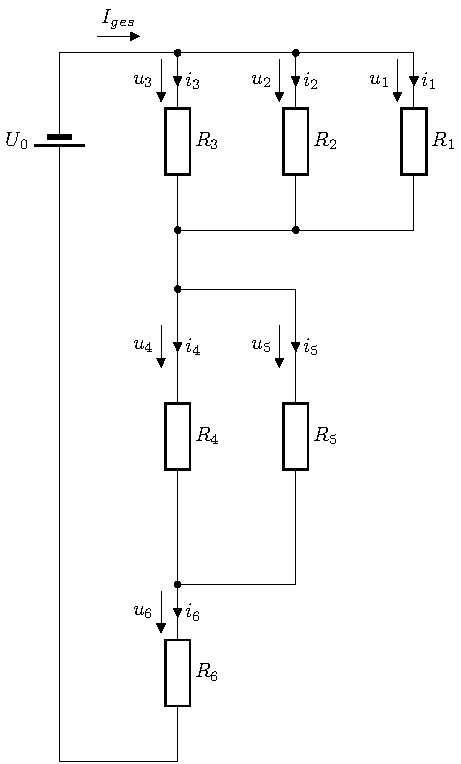
\includegraphics[width=9.3cm]{template_schaltung}
	\end{figure}
\end{question}


{\bigskip {\large \textsl{Viel Erfolg!}}}


\end{document}